% this file is called up by thesis.tex
% content in this file will be fed into the main document

\chapter{Design} % top level followed by section, subsection


% ----------------------- paths to graphics ------------------------

% change according to folder and file names
\ifpdf
    \graphicspath{{7/figures/PNG/}{7/figures/PDF/}{7/figures/}}
\else
    \graphicspath{{7/figures/EPS/}{7/figures/}}
\fi


% ----------------------- contents from here ------------------------
% 

\section{Framework}

% Diagram with overview of different modules and their used as well as
% relationships. Also show integration of open-source technologies.

\begin{figure}
    \centering
	\label{figure:moduledependencies}
	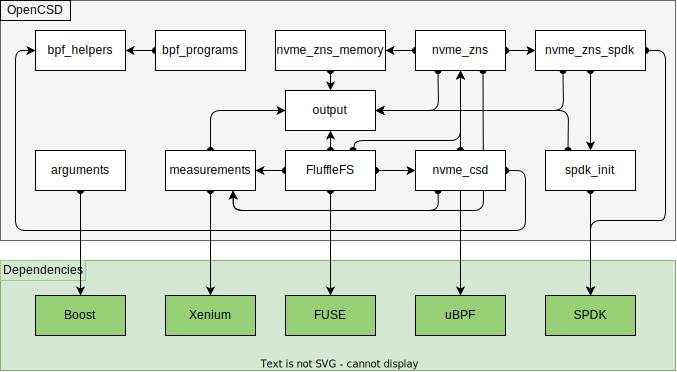
\includegraphics[width=1\textwidth]{resources/images/module-dependencies.pdf}
	\caption{Overview of all OpenCSD components and their depends-on relations}
    % \includesvg[width=0.6\columnwidth]{resources/images/module-dependencies}
\end{figure}

\section{Filesystem}

% Two write pointers, one for RANDOM ZONE and one for LOG ZONE. Use of ZNS is
% optional but allows for lower write-amplification and more explicit garbage
% collection

\subsection{Concurrency}

\section{Offloading}

% Filesystem extended attributes, PID + INODE


% ---------------------------------------------------------------------------
% ----------------------- end of thesis sub-document ------------------------
% ---------------------------------------------------------------------------